\message{ !name(trabalho_final.tex)}%% abtex2-modelo-trabalho-academico.tex, v-1.9.2 laurocesar
%% Copyright 2012-2014 by abnTeX2 group at http://abntex2.googlecode.com/ 
%%
%% This work may be distributed and/or modified under the
%% conditions of the LaTeX Project Public License, either version 1.3
%% of this license or (at your option) any later version.
%% The latest version of this license is in
%%   http://www.latex-project.org/lppl.txt
%% and version 1.3 or later is part of all distributions of LaTeX
%% version 2005/12/01 or later.
%%
%% This work has the LPPL maintenance status `maintained'.
%% 
%% The Current Maintainer of this work is the abnTeX2 team, led
%% by Lauro César Araujo. Further information are available on 
%% http://abntex2.googlecode.com/
%%
%% This work consists of the files abntex2-modelo-trabalho-academico.tex,
%% abntex2-modelo-include-comandos and abntex2-modelo-references.bib
%%

% ------------------------------------------------------------------------
% ------------------------------------------------------------------------
% abnTeX2: Modelo de Trabalho Academico (tese de doutorado, dissertacao de
% mestrado e trabalhos monograficos em geral) em conformidade com 
% ABNT NBR 14724:2011: Informacao e documentacao - Trabalhos academicos -
% Apresentacao
% ------------------------------------------------------------------------
% ------------------------------------------------------------------------

%-------------------------------------------------------------------------
% Modelo adaptado especificamente para o contexto do PPgSI-EACH-USP por 
% Marcelo Fantinato, com auxílio dos Professores Norton T. Roman, Helton
% H. Bíscaro e Sarajane M. Peres, em 2015, com muitos agradecimentos aos 
% criadores da classe e do modelo base.
%
% 20/06/2017: inclusão de "lista de quadros" com base no especificado em:
% https://github.com/abntex/abntex2/wiki/HowToCriarNovoAmbienteListing,
% de autoria de "Eduardo de Santana Medeiros Alexandre".
%
%-------------------------------------------------------------------------

\documentclass[
	% -- opções da classe memoir --
	12pt,				% tamanho da fonte
	% openright,			% capítulos começam em pág ímpar (insere página vazia caso preciso)
	oneside,			% para impressão apenas no anverso (apenas frente). Oposto a twoside
	a4paper,			% tamanho do papel. 
	% -- opções da classe abntex2 --
	%chapter=TITLE,		% títulos de capítulos convertidos em letras maiúsculas
	%section=TITLE,		% títulos de seções convertidos em letras maiúsculas
	%subsection=TITLE,	% títulos de subseções convertidos em letras maiúsculas
	%subsubsection=TITLE,% títulos de subsubseções convertidos em letras maiúsculas
	% -- opções do pacote babel --
	english,			% idioma adicional para hifenização
	%french,				% idioma adicional para hifenização
	%spanish,			% idioma adicional para hifenização
	brazil				% o último idioma é o principal do documento
	]{abntex2ppgsi}

% ---
% Pacotes básicos 
% ---
% \usepackage{lmodern}			% Usa a fonte Latin Modern			
% \usepackage[T1]{fontenc}		% Selecao de codigos de fonte.
\usepackage[utf8]{inputenc}		% Codificacao do documento (conversão automática dos acentos)
\usepackage{lastpage}			% Usado pela Ficha catalográfica
\usepackage{indentfirst}		% Indenta o primeiro parágrafo de cada seção.
\usepackage{color}				% Controle das cores
\usepackage{graphicx}			% Inclusão de gráficos
\usepackage{microtype} 			% para melhorias de justificação
\usepackage{pdfpages}     %para incluir pdf
\usepackage{algorithm}			%para ilustrações do tipo algoritmo
\usepackage{mdwlist}			%para itens com espaço padrão da abnt
\usepackage[noend]{algpseudocode}			%para ilustrações do tipo algoritmo
		
% ---
% Pacotes adicionais, usados apenas no âmbito do Modelo Canônico do abnteX2
% ---
\usepackage{lipsum}				% para geração de dummy text
\usepackage{siunitx}                     %para formatacao numerica
\usepackage[bottom]{footmisc}            % pacote para anotacoes de rodape
% ---

% ---
% Pacotes de citações
% ---
\usepackage[brazilian,hyperpageref]{backref}	 % Paginas com as citações na bibl
\usepackage[alf,abnt-etal-list=0,abnt-etal-text=it]{abntex2cite}	% Citações padrão ABNT

% --- 
% CONFIGURAÇÕES DE PACOTES
% --- 

% ---
% Configurações do pacote backref
% Usado sem a opção hyperpageref de backref
\renewcommand{\backrefpagesname}{Citado na(s) página(s):~}
% Texto padrão antes do número das páginas
\renewcommand{\backref}{}
% Define os textos da citação
\renewcommand*{\backrefalt}[4]{
	\ifcase #1 %
		Nenhuma citação no texto.%
	\or
		Citado na página #2.%
	\else
		Citado #1 vezes nas páginas #2.%
	\fi}%
% ---

% ---
% Informações de dados para CAPA e FOLHA DE ROSTO
% ---

%-------------------------------------------------------------------------
% Comentário adicional do PPgSI - Informações sobre o ``instituicao'':
%
% Não mexer. Deixar exatamente como está.
%
%-------------------------------------------------------------------------
\instituicao{
	UNIVERSIDADE DE SÃO PAULO
	\par
	ESCOLA DE ARTES, CIÊNCIAS E HUMANIDADES
	\par
	PROGRAMA DE PÓS-GRADUAÇÃO EM SISTEMAS DE INFORMAÇÃO}

%-------------------------------------------------------------------------
% Comentário adicional do PPgSI - Informações sobre o ``título'':
%
% Em maiúscula apenas a primeira letra da sentença (do título), exceto 
% nomes próprios, geográficos, institucionais ou Programas ou Projetos ou 
% siglas, os quais podem ter letras em maiúscula também.
%
% O subtítulo do trabalho é opcional.
% Sem ponto final.
%
% Atenção: o título da Dissertação na versão corrigida não pode mudar. 
% Ele deve ser idêntico ao da versão original.
%
%-------------------------------------------------------------------------
\titulo{Título do trabalho: subtítulo do trabalho}

%-------------------------------------------------------------------------
% Comentário adicional do PPgSI - Informações sobre o ``autor'':
%
% Todas as letras em maiúsculas.
% Nome completo.
% Sem ponto final.
%-------------------------------------------------------------------------
\autor{\uppercase{Lucas Freire Lima}}

%-------------------------------------------------------------------------
% Comentário adicional do PPgSI - Informações sobre o ``local'':
%
% Não incluir o ``estado''.
% Sem ponto final.
%-------------------------------------------------------------------------
\local{São Paulo}

%-------------------------------------------------------------------------
% Comentário adicional do PPgSI - Informações sobre a ``data'':
%
% Colocar o ano do depósito (ou seja, o ano da entrega) da respectiva 
% versão, seja ela a versão original (para a defesa) seja ela a versão 
% corrigida (depois da aprovação na defesa). 
%
% Atenção: Se a versão original for depositada no final do ano e a versão 
% corrigida for entregue no ano seguinte, o ano precisa ser atualizado no 
% caso da versão corrigida. 
% Cuidado, pois o ano da ``capa externa'' também precisa ser atualizado 
% nesse caso.
%
% Não incluir o dia, nem o mês.
% Sem ponto final.
%-------------------------------------------------------------------------
\data{2018}

%-------------------------------------------------------------------------
% Comentário adicional do PPgSI - Informações sobre o ``Orientador'':
%
% Se for uma professora, trocar por ``Profa. Dra.''
% Nome completo.
% Sem ponto final.
%-------------------------------------------------------------------------
\orientador{Prof. Dr. Sarajane Marques Peres}

%-------------------------------------------------------------------------
% Comentário adicional do PPgSI - Informações sobre o ``Coorientador'':
%
% Opcional. Incluir apenas se houver co-orientador formal, de acordo com o 
% Regulamento do Programa.
%
% Se for uma professora, trocar por ``Profa. Dra.''
% Nome completo.
% Sem ponto final.
%-------------------------------------------------------------------------
%\coorientador{Prof. Dr. Fulano de Tal}

\tipotrabalho{Dissertação (Mestrado)}

\preambulo{
%-------------------------------------------------------------------------
% Comentário adicional do PPgSI - Informações sobre o texto ``Versão 
% original'':
%
% Não usar para Qualificação.
% Não usar para versão corrigida de Dissertação.
%
%-------------------------------------------------------------------------
Versão original \newline \newline \newline 
%-------------------------------------------------------------------------
% Comentário adicional do PPgSI - Informações sobre o ``texto principal do
% preambulo'':
%
% Para Qualificação, trocar por: Texto de Exame de Qualificação apresentado à Escola de Artes, Ciências e Humanidades da Universidade de São Paulo como parte dos requisitos para obtenção do título de Mestre em Ciências pelo Programa de Pós-graduação em Sistemas de Informação.
%
%-------------------------------------------------------------------------
Dissertação apresentada à Escola de Artes, Ciências e Humanidades da Universidade de São Paulo para obtenção do título de Mestre em Ciências pelo Programa de Pós-graduação em Sistemas de Informação. 
%
\newline \newline Área de concentração: Metodologia e Técnicas da Computação
%-------------------------------------------------------------------------
% Comentário adicional do PPgSI - Informações sobre o texto da ``Versão 
% corrigida'':
%
% Não usar para Qualificação.
% Não usar para versão original de Dissertação.
% 
% Substituir ``xx de xxxxxxxxxxxxxxx de xxxx'' pela ``data da defesa''.
%
%-------------------------------------------------------------------------
\newline \newline \newline Versão corrigida contendo as alterações solicitadas pela comissão julgadora em xx de xxxxxxxxxxxxxxx de xxxx. A versão original encontra-se em acervo reservado na Biblioteca da EACH-USP e na Biblioteca Digital de Teses e Dissertações da USP (BDTD), de acordo com a Resolução CoPGr 6018, de 13 de outubro de 2011.}
% ---


% ---
% Configurações de aparência do PDF final

% alterando o aspecto da cor azul
\definecolor{blue}{RGB}{41,5,195}

% informações do PDF
\makeatletter
\hypersetup{
     	%pagebackref=true,
		pdftitle={\@title}, 
		pdfauthor={\@author},
    	pdfsubject={\imprimirpreambulo},
	    pdfcreator={LaTeX com abnTeX2 adaptado para o PPgSI-EACH-USP},
		pdfkeywords={abnt}{latex}{abntex}{abntex2}{qualificação de mestrado}{dissertação de mestrado}{ppgsi}, 
		colorlinks=true,       		% false: boxed links; true: colored links
    	linkcolor=black,          	% color of internal links
    	citecolor=black,        		% color of links to bibliography
    	filecolor=black,      		% color of file links
		urlcolor=black,
		bookmarksdepth=4
}
\makeatother
% --- 

% --- 
% Espaçamentos entre linhas e parágrafos 
% --- 

% O tamanho do parágrafo é dado por:
\setlength{\parindent}{1.25cm}

% Controle do espaçamento entre um parágrafo e outro:
\setlength{\parskip}{0cm}  % tente também \onelineskip
\renewcommand{\baselinestretch}{1.5}

% ---
% compila o indice
% ---
\makeindex
% ---

	% Controlar linhas orfas e viuvas
  \clubpenalty10000
  \widowpenalty10000
  \displaywidowpenalty10000


\gdef\clearforchapter{}

% ----
% Início do documento
% ----
\begin{document}

\message{ !name(trabalho_final.tex) !offset(-3) }


% Retira espaço extra obsoleto entre as frases.
\frenchspacing

% ----------------------------------------------------------
% ELEMENTOS PRÉ-TEXTUAIS
% ----------------------------------------------------------
% \pretextual

% ---
% Capa
% ---
%-------------------------------------------------------------------------
% Comentário adicional do PPgSI - Informações sobre a ``capa'':
%
% Esta é a ``capa'' principal/oficial do trabalho, a ser impressa apenas 
% para os casos de encadernação simples (ou seja, em ``espiral'' com 
% plástico na frente).
% 
% Não imprimir esta ``capa'' quando houver ``capa dura'' ou ``capa brochura'' 
% em que estas mesmas informações já estão presentes nela.
%
%-------------------------------------------------------------------------
%\imprimircapa
% ---

% ---
% Folha de rosto
% (o * indica que haverá a ficha bibliográfica)
% ---
%\imprimirfolhaderosto*
% ---

% ---
% Inserir a autorização para reprodução e ficha bibliografica
% ---

%-------------------------------------------------------------------------
% Comentário adicional do PPgSI - Informações sobre o texto da 
% ``autorização para reprodução e ficha bibliografica'':
%
% Página a ser usada apenas para Dissertação (tanto na versão original 
% quanto na versão corrigida).
%
% Solicitar a ficha catalográfica na Biblioteca da EACH. 
% Duas versões devem ser solicitadas, em dois momentos distintos: uma vez 
% para a versão original, e depois outra atualizada para a versão 
% corrigida.
%
% Atenção: esta página de ``autorização para reprodução e ficha 
% catalográfica'' deve ser impressa obrigatoriamente no verso da folha de 
% rosto.
%
% Não usar esta página para Qualificação.
%
% Substitua o arquivo ``fig_ficha_catalografica.pdf'' abaixo referenciado 
% pelo PDF elaborado pela Biblioteca
%
%-------------------------------------------------------------------------
% \begin{fichacatalografica}
%     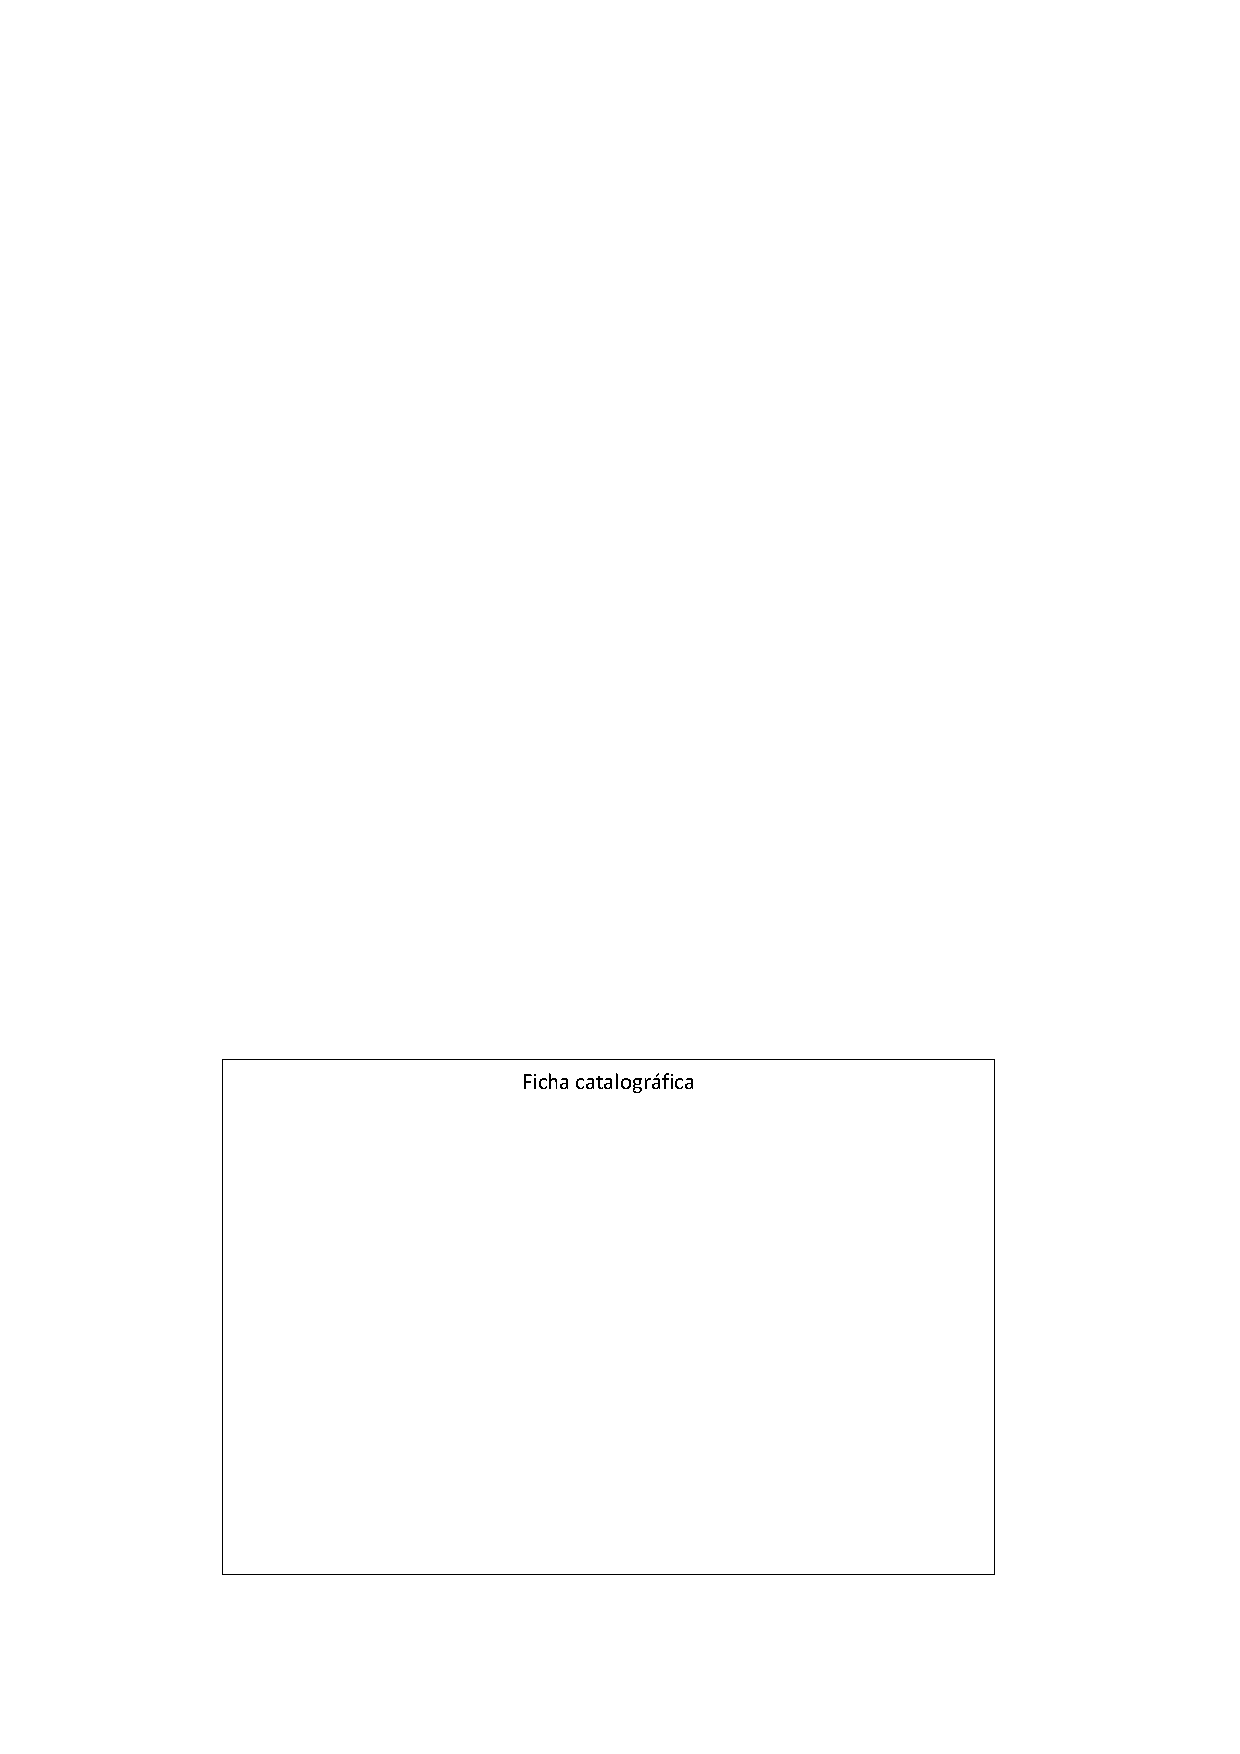
\includepdf{fig_ficha_catalografica.pdf}
% \end{fichacatalografica}

% ---
% Inserir errata
% ---
%-------------------------------------------------------------------------
% Comentário adicional do PPgSI - Informações sobre ``Errata'':
%
% Usar esta página de errata apenas em casos de excepcionais, e apenas 
% para a versão corrigida da Dissertação. Por exemplo, quando depois de
% já depositada e publicada a versão corrigida, ainda assim verifica-se
% a necessidade de alguma correção adicional.
%
% Se precisar usar esta página, busque a forma correta (o modelo correto) 
% para fazê-lo, de acordo com a norma ABNT.
%
% Não usar esta página para versão original de Dissertação.
% Não usar esta página para Qualificação.
%
%-------------------------------------------------------------------------
% \begin{errata}
% Elemento opcional para versão corrigida, depois de depositada.
% \end{errata}
% ---

% ---
% Inserir folha de aprovação
% ---

% \begin{folhadeaprovacao}
% %-------------------------------------------------------------------------
% % Comentário adicional do PPgSI - Informações sobre ``Folha da aprovação'':
% %
% % Página a ser usada apenas para Dissertação.
% %
% % Não usar esta página para Qualificação.
% %
% % Substituir ``Fulano de Tal'' pelo nome completo do autor do trabalho, com 
% % apenas as iniciais em maiúsculo.
% %
% % Substituir ``___ de ______________ de ______'' por: 
% %     - Para versão original de Dissertação: deixar em branco, pois a data 
% %       pode mudar, mesmo que ela já esteja prevista.
% %     - Para versão corrigida de Dissertação: usar a data em que a defesa 
% %       efetivamente ocorreu.
% %
% %-------------------------------------------------------------------------
% \noindent Dissertação de autoria de Fulano de Tal, sob o título \textbf{``\imprimirtitulo''}, apresentada à Escola de Artes, Ciências e Humanidades da Universidade de São Paulo, para obtenção do título de Mestre em Ciências pelo Programa de Pós-graduação em Sistemas de Informação, na área de concentração Metodologia e Técnicas da Computação, aprovada em \_\_\_\_\_\_\_ de \_\_\_\_\_\_\_\_\_\_\_\_\_\_\_\_\_\_\_\_\_\_ de \_\_\_\_\_\_\_\_\_\_ pela comissão julgadora constituída pelos doutores:

% \vspace*{3cm}

% \begin{center}
% %-------------------------------------------------------------------------
% % Comentário adicional do PPgSI - Informações sobre ``assinaturas'':
% %
% % Para versão original de Dissertação: deixar em 
% % branco (ou seja, assim como está abaixo), pois os membros da banca podem
% % mudar, mesmo que eles já estejam previstos.
% % 
% % Para versão corrigida de Dissertação: usar os dados dos examinadores que 
% % efetivamente participaram da defesa. 
% % 
% % Para versão corrigida de Dissertação: em caso de ``professora'', trocar 
% % por ``Profa. Dra.'' 
% % 
% % Para versão corrigida de Dissertação: ao colocar os nomes dos 
% % examinadores, remover o sublinhado
% % 
% % Para versão corrigida de Dissertação: ao colocar os nomes dos 
% % examinadores, usar seus nomes completos, exatamente conforme constam em 
% % seus Currículos Lattes
% % 
% % Para versão corrigida de Dissertação: ao colocar os nomes das 
% % instituições, remover o sublinhado e remover a palavra ``Instituição:''
% %
% % Não abreviar os nomes das instituições.
% %
% %-------------------------------------------------------------------------
% \_\_\_\_\_\_\_\_\_\_\_\_\_\_\_\_\_\_\_\_\_\_\_\_\_\_\_\_\_\_\_\_\_\_\_\_\_\_\_\_\_\_\_\_\_\_\_\_\_\_\_\_\_\_\_\_
% \vspace*{0.2cm} 
% \\ \textbf{Prof. Dr. \_\_\_\_\_\_\_\_\_\_\_\_\_\_\_\_\_\_\_\_\_\_\_\_\_\_\_\_\_\_\_\_\_\_\_\_\_\_\_\_\_\_\_\_\_\_\_\_\_\_\_\_\_\_\_\_\_\_\_\_\_\_} 
% \\ \vspace*{0.2cm} 
% Instituição: \_\_\_\_\_\_\_\_\_\_\_\_\_\_\_\_\_\_\_\_\_\_\_\_\_\_\_\_\_\_\_\_\_\_\_\_\_\_\_\_\_\_\_\_\_\_\_\_\_\_\_\_\_\_\_\_\_\_ 
% \\ \vspace*{0.2cm}
% Presidente 

% \vspace*{2cm}

% \_\_\_\_\_\_\_\_\_\_\_\_\_\_\_\_\_\_\_\_\_\_\_\_\_\_\_\_\_\_\_\_\_\_\_\_\_\_\_\_\_\_\_\_\_\_\_\_\_\_\_\_\_\_\_\_
% \vspace*{0.2cm} 
% \\ \textbf{Prof. Dr. \_\_\_\_\_\_\_\_\_\_\_\_\_\_\_\_\_\_\_\_\_\_\_\_\_\_\_\_\_\_\_\_\_\_\_\_\_\_\_\_\_\_\_\_\_\_\_\_\_\_\_\_\_\_\_\_\_\_\_\_\_\_} 
% \\ \vspace*{0.2cm} 
% Instituição: \_\_\_\_\_\_\_\_\_\_\_\_\_\_\_\_\_\_\_\_\_\_\_\_\_\_\_\_\_\_\_\_\_\_\_\_\_\_\_\_\_\_\_\_\_\_\_\_\_\_\_\_\_\_\_\_\_\_

% \vspace*{2cm}

% \_\_\_\_\_\_\_\_\_\_\_\_\_\_\_\_\_\_\_\_\_\_\_\_\_\_\_\_\_\_\_\_\_\_\_\_\_\_\_\_\_\_\_\_\_\_\_\_\_\_\_\_\_\_\_\_
% \vspace*{0.2cm} 
% \\ \textbf{Prof. Dr. \_\_\_\_\_\_\_\_\_\_\_\_\_\_\_\_\_\_\_\_\_\_\_\_\_\_\_\_\_\_\_\_\_\_\_\_\_\_\_\_\_\_\_\_\_\_\_\_\_\_\_\_\_\_\_\_\_\_\_\_\_\_} 
% \\ \vspace*{0.2cm} 
% Instituição: \_\_\_\_\_\_\_\_\_\_\_\_\_\_\_\_\_\_\_\_\_\_\_\_\_\_\_\_\_\_\_\_\_\_\_\_\_\_\_\_\_\_\_\_\_\_\_\_\_\_\_\_\_\_\_\_\_\_

% \vspace*{2cm}

% \_\_\_\_\_\_\_\_\_\_\_\_\_\_\_\_\_\_\_\_\_\_\_\_\_\_\_\_\_\_\_\_\_\_\_\_\_\_\_\_\_\_\_\_\_\_\_\_\_\_\_\_\_\_\_\_
% \vspace*{0.2cm} 
% \\ \textbf{Prof. Dr. \_\_\_\_\_\_\_\_\_\_\_\_\_\_\_\_\_\_\_\_\_\_\_\_\_\_\_\_\_\_\_\_\_\_\_\_\_\_\_\_\_\_\_\_\_\_\_\_\_\_\_\_\_\_\_\_\_\_\_\_\_\_} 
% \\ \vspace*{0.2cm} 
% Instituição: \_\_\_\_\_\_\_\_\_\_\_\_\_\_\_\_\_\_\_\_\_\_\_\_\_\_\_\_\_\_\_\_\_\_\_\_\_\_\_\_\_\_\_\_\_\_\_\_\_\_\_\_\_\_\_\_\_\_

% \end{center}
  
% \end{folhadeaprovacao}
% ---

% ---
% Dedicatória
% ---
%-------------------------------------------------------------------------
% Comentário adicional do PPgSI - Informações sobre ``Dedicatória'': 
%
% Opcional para Dissertação.
% Não sugerido para Qualificação.
% 
%-------------------------------------------------------------------------
% \begin{dedicatoria}
%    \vspace*{\fill}
%    \centering
%    \noindent
%    \textit{Escreva aqui sua dedicatória, se desejar, ou remova esta página...} 
% 	 \vspace*{\fill}
% \end{dedicatoria}
% ---

% ---
% Agradecimentos
% ---
%-------------------------------------------------------------------------
% Comentário adicional do PPgSI - Informações sobre ``Agradecimentos'': 
%
% Opcional para Dissertação.
% Não sugerido para Qualificação.
% 
% Lembrar de agradecer agências de fomento e outras instituições similares.
%
%-------------------------------------------------------------------------
% \begin{agradecimentos}
% Texto de exemplo, texto de exemplo, texto de exemplo, texto de exemplo, texto de exemplo, texto de exemplo, texto de exemplo, texto de exemplo, texto de exemplo, texto de exemplo, texto de exemplo, texto de exemplo, texto de exemplo, texto de exemplo, texto de exemplo, texto de exemplo, texto de exemplo, texto de exemplo, texto de exemplo, texto de exemplo, texto de exemplo, texto de exemplo.

% Texto de exemplo, texto de exemplo, texto de exemplo, texto de exemplo, texto de exemplo, texto de exemplo, texto de exemplo, texto de exemplo, texto de exemplo, texto de exemplo, texto de exemplo, texto de exemplo, texto de exemplo, texto de exemplo, texto de exemplo, texto de exemplo, texto de exemplo, texto de exemplo, texto de exemplo, texto de exemplo, texto de exemplo, texto de exemplo.

% Texto de exemplo, texto de exemplo, texto de exemplo, texto de exemplo, texto de exemplo, texto de exemplo, texto de exemplo, texto de exemplo, texto de exemplo, texto de exemplo, texto de exemplo, texto de exemplo, texto de exemplo, texto de exemplo, texto de exemplo, texto de exemplo, texto de exemplo, texto de exemplo, texto de exemplo, texto de exemplo, texto de exemplo, texto de exemplo.

% Texto de exemplo, texto de exemplo, texto de exemplo, texto de exemplo, texto de exemplo, texto de exemplo, texto de exemplo, texto de exemplo, texto de exemplo, texto de exemplo, texto de exemplo, texto de exemplo, texto de exemplo, texto de exemplo, texto de exemplo, texto de exemplo, texto de exemplo, texto de exemplo, texto de exemplo, texto de exemplo, texto de exemplo, texto de exemplo.

% Texto de exemplo, texto de exemplo, texto de exemplo, texto de exemplo, texto de exemplo, texto de exemplo, texto de exemplo, texto de exemplo, texto de exemplo, texto de exemplo, texto de exemplo, texto de exemplo, texto de exemplo, texto de exemplo, texto de exemplo, texto de exemplo, texto de exemplo, texto de exemplo, texto de exemplo, texto de exemplo, texto de exemplo, texto de exemplo.
% \end{agradecimentos}
% ---

% ---
% Epígrafe
% ---
%-------------------------------------------------------------------------
% Comentário adicional do PPgSI - Informações sobre ``Epígrafe'': 
%
% Opcional para Dissertação.
% Não sugerido para Qualificação.
% 
%-------------------------------------------------------------------------
% \begin{epigrafe}
%     \vspace*{\fill}
% 	\begin{flushright}
% 		\textit{``Escreva aqui uma epígrafe, se desejar, ou remova esta página...''\\
% 		(Autor da epígrafe)}
% 	\end{flushright}
% \end{epigrafe}
% ---

% ---
% RESUMOS
% ---

% resumo em português
% \setlength{\absparsep}{18pt} % ajusta o espaçamento dos parágrafos do resumo
% \begin{resumo}

% %-------------------------------------------------------------------------
% % Comentário adicional do PPgSI - Informações sobre ``referência'':
% % 
% % Troque os seguintes campos pelos dados de sua Dissertação (mantendo a 
% % formatação e pontuação):
% %   - SOBRENOME
% %   - Nome1
% %   - Nome2
% %   - Nome3
% %   - Título do trabalho: subtítulo do trabalho
% %   - AnoDeDefesa
% %
% % Mantenha todas as demais informações exatamente como estão.
% % 
% % [Não usar essas informações de ``referência'' para Qualificação]
% %
% %-------------------------------------------------------------------------
% \begin{flushleft}
% SOBRENOME, Nome1 Nome2 Nome3. \textbf{Título do trabalho}: subtítulo do trabalho. \imprimirdata. \pageref{LastPage} f. Dissertação (Mestrado em Ciências) – Escola de Artes, Ciências e Humanidades, Universidade de São Paulo, São Paulo, AnoDeDefesa.
% \end{flushleft}

% Escreva aqui o texto do seu resumo... (redigido em parágrafo único, no máximo em uma página, contendo no ``máximo 500 palavras'', e apresentando um resumo de todos o seu trabalho, incluindo objetivos, metodologia, resultados e conclusões; não inclua apenas a contextualização até chegar nos objetivos, é importante fazer um resumo de todos os capítulos do texto, até chegar à conclusão). Texto de exemplo, texto de exemplo, texto de exemplo, texto de exemplo, texto de exemplo, texto de exemplo, texto de exemplo, texto de exemplo, texto de exemplo, texto de exemplo, texto de exemplo, texto de exemplo, texto de exemplo, texto de exemplo, texto de exemplo, texto de exemplo, texto de exemplo, texto de exemplo, texto de exemplo, texto de exemplo, texto de exemplo, texto de exemplo.

% Palavras-chaves: Palavra1. Palavra2. Palavra3. etc.
% \end{resumo}

% % resumo em inglês
% %-------------------------------------------------------------------------
% % Comentário adicional do PPgSI - Informações sobre ``resumo em inglês''
% % 
% % Caso a Qualificação ou a Dissertação inteira seja elaborada no idioma inglês, 
% % então o ``Abstract'' vem antes do ``Resumo''.
% % 
% %-------------------------------------------------------------------------
% \begin{resumo}[Abstract]
% \begin{otherlanguage*}{english}

% %-------------------------------------------------------------------------
% % Comentário adicional do PPgSI - Informações sobre ``referência em inglês''
% % 
% % Troque os seguintes campos pelos dados de sua Dissertação (mantendo a 
% % formatação e pontuação):
% %     - SURNAME
% %     - FirstName1
% %     - MiddleName1
% %     - MiddleName2
% %     - Work title: work subtitle
% %     - DefenseYear (Ano de Defesa)
% %
% % Mantenha todas as demais informações exatamente como estão.
% %
% % [Não usar essas informações de ``referência'' para Qualificação]
% %
% %-------------------------------------------------------------------------
% \begin{flushleft}
% SURNAME, FirstName MiddleName1 MiddleName2. \textbf{Work title}: work subtitle. \imprimirdata. \pageref{LastPage} p. Dissertation (Master of Science) – School of Arts, Sciences and Humanities, University of São Paulo, São Paulo, DefenseYear. 
% \end{flushleft}

% Write here the English version of your ``Resumo''. Example text, example text, example text, example text, example text, example text, example text, example text, example text, example text, example text, example text, example text, example text, example text, example text, example text, example text, example text, example text, example text, example text, example text, example text, example text, example text, example text, example text, example text, example text, example text, example text, example text, example text, example text, example text, example text, example text, example text, example text, example text, example text, example text, example text, example text, example text, example text.

% Keywords: Keyword1. Keyword2. Keyword3. etc.
% \end{otherlanguage*}
% \end{resumo}

% ---
% ---
% inserir lista de figuras
% ---
% \pdfbookmark[0]{\listfigurename}{lof}
% \listoffigures*
% \cleardoublepage
% % ---

% % ---
% % inserir lista de algoritmos
% % ---
% \pdfbookmark[0]{\listalgorithmname}{loa}
% \listofalgorithms
% \cleardoublepage

% % ---
% % inserir lista de quadros
% % ---
% \pdfbookmark[0]{\listofquadrosname}{loq}
% \listofquadros*
% \cleardoublepage


% % ---
% % inserir lista de tabelas
% % ---
% \pdfbookmark[0]{\listtablename}{lot}
% \listoftables*
% \cleardoublepage
% ---

% ---
% inserir lista de abreviaturas e siglas
% ---
%-------------------------------------------------------------------------
% Comentário adicional do PPgSI - Informações sobre ``Lista de abreviaturas 
% e siglas'': 
%
% Opcional.
% Uma vez que se deseja usar, é necessário manter padrão e consistência no
% trabalho inteiro.
% Se usar: inserir em ordem alfabética.
%
%-------------------------------------------------------------------------
% \begin{siglas}
%   \item[Sigla/abreviatura 1] Definição da sigla ou da abreviatura por extenso
%   \item[Sigla/abreviatura 2] Definição da sigla ou da abreviatura por extenso
%   \item[Sigla/abreviatura 3] Definição da sigla ou da abreviatura por extenso
%   \item[Sigla/abreviatura 4] Definição da sigla ou da abreviatura por extenso
%   \item[Sigla/abreviatura 5] Definição da sigla ou da abreviatura por extenso
%   \item[Sigla/abreviatura 6] Definição da sigla ou da abreviatura por extenso
%   \item[Sigla/abreviatura 7] Definição da sigla ou da abreviatura por extenso
%   \item[Sigla/abreviatura 8] Definição da sigla ou da abreviatura por extenso
%   \item[Sigla/abreviatura 9] Definição da sigla ou da abreviatura por extenso
%   \item[Sigla/abreviatura 10] Definição da sigla ou da abreviatura por extenso
% \end{siglas}
% ---

% ---
% inserir lista de símbolos
% ---
%-------------------------------------------------------------------------
% Comentário adicional do PPgSI - Informações sobre ``Lista de símbolos'': 
%
% Opcional.
% Uma vez que se deseja usar, é necessário manter padrão e consistência no
% trabalho inteiro.
% Se usar: inserir na ordem em que aparece no texto.
% 
%-------------------------------------------------------------------------
% \begin{simbolos}
%   \item[$ \Gamma $] Letra grega Gama
%   \item[$ \Lambda $] Lambda
%   \item[$ \zeta $] Letra grega minúscula zeta
%   \item[$ \in $] Pertence
% \end{simbolos}
% ---

% ---
% inserir o sumario
% ---
% % \pdfbookmark[0]{\contentsname}{toc}
% % \tableofcontents*
% % \cleardoublepage
% ---



% ----------------------------------------------------------
% ELEMENTOS TEXTUAIS
% ----------------------------------------------------------
\textual



%-------------------------------------------------------------------------
% Comentário adicional do PPgSI - Informações sobre ``títulos de seções''
% 
% Para todos os títulos (seções, subseções, tabelas, ilustrações, etc.):
%
% Em maiúscula apenas a primeira letra da sentença (do título), exceto 
% nomes próprios, geográficos, institucionais ou Programas ou Projetos ou
% siglas, os quais podem ter letras em maiúscula também.
%
%-------------------------------------------------------------------------
\chapter{Tema}
Os automóveis representam um importante papel na sociedade atual
sendo aproveitados não somente para locomoção, mas também como meio
de serviço. O Departamento Nacional de Trânsito (DENATRAN), órgão
governamental responsável pelo levantamento da frota de veículos do
território nacional, estima em sua última pesquisa, realizada em abril
de 2018, que o Brasil possui \num{98201128} veículos \cite{DENATRANfrotaabr2018}.

O comportamento de um motorista pode ser
modelado considerando as capacidades do condutor e a
execução da tarefa de direção. A capacidade do condutor caracteriza a parcela biológica do
modelo, sendo responsável pela sua velocidade de processamento, tempo de
reação e seus limites físicos \cite{Fuller2005461}. Este aspecto biológico leva em
consideração a unicidade de cada indivíduo e o seu modo ímpar de
interação com os
instrumentos de condução do veículo. Estas duas características
singulares permitem a formação e a extração de dados biométricos que podem
utilizados para identificar ou validar um condutor de modo não intrusivo.

%Sensores automobilísticos controlam e monitoram a utilização do veículo
%Cada motorista é um ator distinto, pois interage de forma única com os sensores
%A bioassinatura é obtida através da condensação, normalização, análise
%e extração de características dos dados sensoriados

\vspace{1.2cm}
\chapter{Motivação}
Em uma sociedade onde os veículos estão presentes nos mais variados
ramos da atividade econômica, é preciso saber de antemão quem é o
motorista por trás do volante. Contudo, somente essa informação
preliminar isolada não é o
suficiente para prevenir fraudes de identidade. Uma validação não
intrusiva, durante a execução da atividade de direção, é necessária
para aumentar a confiabilidade da informação.

Fazendo uso dos dados sensoriados do veículo que está sob comando do
condutor, o reconhecimento biométrico permite estabelecer a identidade de uma pessoa pela análise de suas características comportamentais
\cite{Nandakumar2008}.

%Por ser um meio não intrusivo de identificação, a biometria pode ser
%utilizada na prevenção à fraudes e roubos

%Por utilizar dados veiculares sensoriados, é um método  não intrusivo
%que pode ser utilizado isoladamente ou em  conjunto com outras soluções de identificação
\vspace{1.2cm}
\chapter{Lacuna}
Os trabalhos mais atuais que contemplam a análise comportamental de
motoristas estão mais preocupados em identificar o estado fisiológico
do condutor como sonolência, distração, agressividade e afins
\cite{Al-Sultan20134264,Liang20071,Gindele201569,Chong2013207}. Poucos
trabalhos como os de \cite{Liang2014146,Liu2018,Lee2017} foram
desenvolvidos com o objetivo principal de analisar o perfil do
motorista de forma não intrusiva, empregando os dados sensoriados em
tempo real provenientes do veículo, e aplicando técnicas de \textit{deep learning}.

%Atualmente, a análise do perfil de condução de um motorista preocupa-se em inferir o seu estado fisiológico
%Existem poucos estudos que utilizam os mesmos dados sensoriados para
%inferir a identidade do motorista, de forma não intrusiva, e classificá-lo dentro de um grupo

\vspace{1.2cm}
\chapter{Objetivo}
Apresentar um modelo, que contemple o uso de dados sensoriados do
veículo extraídos em tempo real, com o intuito de realizar a análise
comportamental do motorista durante a execução da tarefa de
direção. Além da tarefa descrita anteriormente, o modelo deve ser apto
à identificar o motorista com base no seu perfil de condução, gerado na
tarefa anterior, empregando técnicas de \textit{deep learning}.

%Confeccionar um modelo para inferência da identidade do condutor
%veicular utilizando a sua bioassinatura de condução em conjunto com os
%dados sensoriados instantâneos do veículo.

\vspace{1.2cm}
\chapter{Hipótese}
Espera-se que com o uso de técnicas de aprendizagem profunda
(\textit{deep learning}), que são capazes de trabalhar em conjunto com séries temporais de alta
dimensionalidade e em tempo real, seja possível obter
resultados mais apurados ao realizar a extração de características e
a identificação biométrica do motorista através do seu comportamento de
direção. Tais técnicas devem apresentar melhores índices de sucesso no
uso dos métodos \textit{f-score} e curvas \textit{ROC}, quando
comparados aos resultados obtidos aplicando-se técnicas de aprendizado superficial (\textit{shallow learning}).

Além da expectativa acima, almeja-se que o custo computacional para a
execução de tais atividades e sua operacionalização não inviabilize a
sua utilização pelo mercado.

\vspace{1.2cm}
\chapter{Justificativa}
Caso a aplicação da técnica de aprendizagem profunda apresente os
resultados esperados, será possível explorar novas maneiras para
criar-se perfis comportamentais não intrusivos

\vspace{1.2cm}
\chapter{Metodologia}
Pesquisa quantitativa
Utilização de dados reais captados por sensores
  Geração das bioassinaturas, testes e validação das mesmas
  Inferência do motorista
Utilização de métodos de aprendizagem profunda
  Geração das bioassinaturas
  Inferência da identidade em tempo real
  Análise estatística para avaliação dos resultados obtidos\par

  \begin{figure}[H]
    \centering
    \caption{Cronograma de execução das atividades.}
    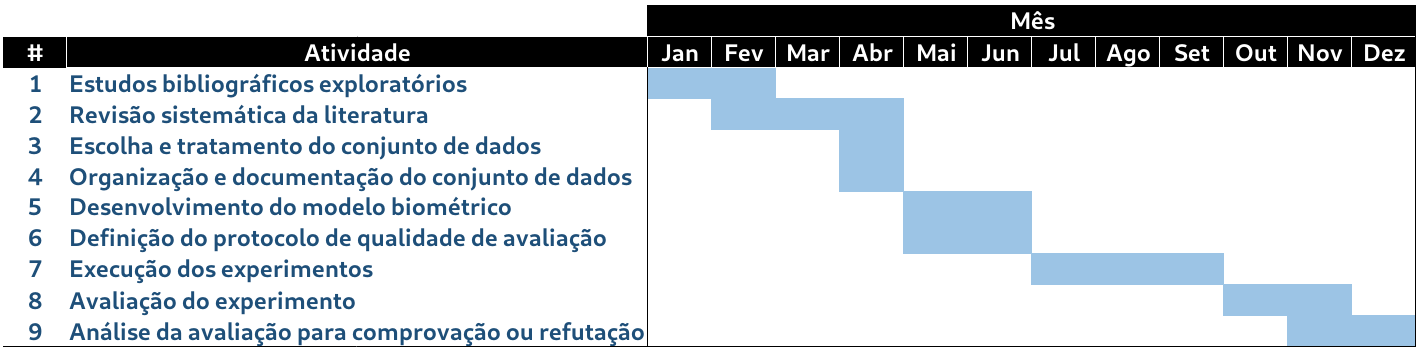
\includegraphics[scale=1.46]{static/cronograma}
    \source{Lucas Freire Lima, 2018}
  \end{figure}

\vspace{1.2cm}  
\chapter{Avaliação}
Geração das bioassinaturas
  Comparação do tempo de execução e custo computacional
  Complexidade de aplicação do método de geração
Inferência do condutor
  f-score
  Tempo médio para convergência e custo computacional

Escolha do “melhor modelo”
Razão ponderada entre os resultados obtidos

\vspace{1.2cm}
\chapter{Contribuições e Limitações}
\section{Contribuições}
Modelo para geração e validação de bioassinaturas veiculares
Alternativa aos métodos de identificação intrusivos
\section{Limitações}
Restrição a um tipo de veículo
Limitação a motoristas experientes
Não há classificação das rotas

\pagebreak

% ----------------------------------------------------------
% ELEMENTOS PÓS-TEXTUAIS
% ----------------------------------------------------------
\postextual
% ----------------------------------------------------------

% ----------------------------------------------------------
% Referências bibliográficas
% ----------------------------------------------------------
\bibliography{referencias}

% ----------------------------------------------------------
% Glossário
% ----------------------------------------------------------
%
% Consulte o manual da classe abntex2 para orientações sobre o glossário.
%
%\glossary

%---------------------------------------------------------------------
% INDICE REMISSIVO
%---------------------------------------------------------------------
%%%%%MF\phantompart
%%%%%MF\printindex
%---------------------------------------------------------------------

\end{document}

%%% Local Variables:
%%% mode: latex
%%% TeX-master: t
%%% End:

\message{ !name(trabalho_final.tex) !offset(-878) }
